\section{Lecture 15: Wrapping Up QAOA: Intro to Coding in PennyLane,
QUBO}\label{sec:lecture15}

\subsection*{Review}

\qs{QAOA Circuit}{
  What are the main components of a QAOA circuit and how are they arranged?
}

\sol{
  A QAOA circuit consists of:
  \begin{enumerate}
    \item Initial state preparation: Apply Hadamard gates to create equal
      superposition $H^{\otimes n}|0\rangle^{\otimes n}$

    \item $P$ alternating layers of:
      \begin{itemize}
        \item Cost operator: $e^{-i\gamma_p H_C}$ which encodes the problem's
          objective function

        \item Mixer operator: $e^{-i\beta_p H_M}$ which explores the solution
          space
      \end{itemize}

    \item Final measurement in the computational basis
  \end{enumerate}
}

\vspace{0.3cm}

\index{Quantum Approximate Optimization Algorithms!PennyLane}
\subsection*{PennyLane}

\dfn{PennyLane}{PennyLane is an open-source software framework for quantum
  machine learning, quantum computing, and quantum chemistry. It enables users
  to train quantum circuits in the same way as neural networks, using automatic
differentiation techniques from machine learning.}

\vspace{0.3cm}

\noindent
\textbf{Key Features of PennyLane:}
\begin{itemize}
  \item \textbf{Hybrid quantum-classical computation}: Seamlessly connects
    classical machine learning libraries with quantum processing units

  \item \textbf{Automatic differentiation}: Computes gradients of quantum
    circuits for optimization tasks

  \item \textbf{Hardware agnostic}: Works with multiple quantum computing
    platforms and simulators

  \item \textbf{Built-in optimizers}: Includes various classical optimization
    algorithms

  \item \textbf{Quantum machine learning toolkit}: Provides implementations
    of common quantum algorithms and models
\end{itemize}

\begin{figure}[H]
  \centering
  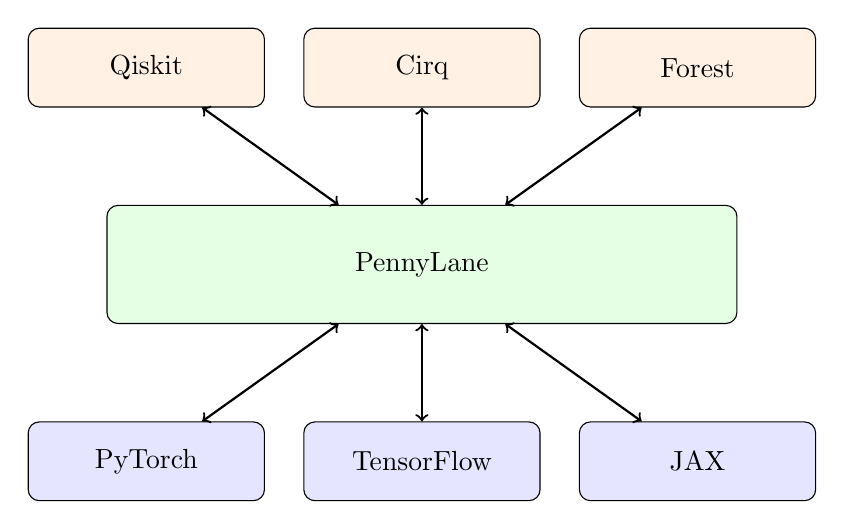
\begin{tikzpicture}
    \node[draw, rounded corners, fill=green!10, minimum width=8cm, minimum height=1.5cm] (pennylane) at (0,0) {PennyLane};

    \node[draw, rounded corners, fill=blue!10, minimum width=3cm, minimum height=1cm] (pytorch) at (-3.5,-2.5) {PyTorch};
    \node[draw, rounded corners, fill=blue!10, minimum width=3cm, minimum height=1cm] (tensorflow) at (0,-2.5) {TensorFlow};
    \node[draw, rounded corners, fill=blue!10, minimum width=3cm, minimum height=1cm] (jax) at (3.5,-2.5) {JAX};

    \node[draw, rounded corners, fill=orange!10, minimum width=3cm, minimum height=1cm] (qiskit) at (-3.5,2.5) {Qiskit};
    \node[draw, rounded corners, fill=orange!10, minimum width=3cm, minimum height=1cm] (cirq) at (0,2.5) {Cirq};
    \node[draw, rounded corners, fill=orange!10, minimum width=3cm, minimum height=1cm] (forest) at (3.5,2.5) {Forest};

    \draw[<->, thick] (pennylane) -- (pytorch);
    \draw[<->, thick] (pennylane) -- (tensorflow);
    \draw[<->, thick] (pennylane) -- (jax);

    \draw[<->, thick] (pennylane) -- (qiskit);
    \draw[<->, thick] (pennylane) -- (cirq);
    \draw[<->, thick] (pennylane) -- (forest);
  \end{tikzpicture}
  \caption{PennyLane connects classical ML frameworks with quantum computing
  platforms}
  \label{fig:pennylane-ecosystem}
\end{figure}

\vspace{0.3cm}

\noindent
\textbf{Basic Structure of a PennyLane Program:}
\begin{enumerate}
  \item Define a quantum device

  \item Create a quantum circuit using a QNode decorator

  \item Define a cost function

  \item Optimize the circuit parameters
\end{enumerate}

\begin{minted}{python}
  # Basic PennyLane workflow
  import pennylane as qml
  from pennylane import numpy as np

  # 1. Define a device
  dev = qml.device("default.qubit", wires=4)

  # 2. Define a quantum circuit (QNode)
  @qml.qnode(dev)
  def circuit(params):
  # Prepare initial state
  for i in range(4):
  qml.Hadamard(wires=i)

  # Apply parameterized gates
  qml.RX(params[0], wires=0)
  qml.RY(params[1], wires=1)

  # Return expectation values
  return qml.expval(qml.PauliZ(0))

  # 3. Run the circuit
  params = np.array([0.1, 0.2], requires_grad=True)
  result = circuit(params)
\end{minted}

\vspace{0.3cm}

\paragraph{QAOA Implementation in PennyLane} Here's how to implement QAOA for
MaxCut in PennyLane:

\begin{minted}{python}
  import pennylane as qml
  import networkx as nx
  from pennylane import numpy as np

  # Define the graph
  edges = [(0, 1), (0, 2), (0, 3), (1, 2), (2, 3)]
  graph = nx.Graph(edges)

  # Get the MaxCut cost and mixer Hamiltonians
  C, B = qml.qaoa.maxcut(graph)

  # Define the number of layers
  L = 1
  num_qubits = 4
  qubits = range(num_qubits)

  # Define the QAOA layers
  def qaoa_layer(gamma, beta):
  qml.qaoa.cost_layer(gamma, C)
  qml.qaoa.mixer_layer(beta, B)

  # Define the full circuit
  def circuit(params, **kwargs):
  for qubit in qubits:
  qml.Hadamard(wires=qubit)
  qml.layer(qaoa_layer, L, params[0], params[1])

  # Create a quantum device
  dev = qml.device("default.qubit", wires=qubits)

  # Define the cost function
  @qml.qnode(dev)
  def cost_function(params):
  circuit(params)
  return qml.expval(C)

  # Optimize the parameters
  optimizer = qml.AdagradOptimizer(stepsize=0.1)
  steps = 50
  params = np.array([[np.random.random()*2*np.pi],
  [np.random.random()*2*np.pi]],
  requires_grad=True)

  for i in range(steps):
  params = optimizer.step(cost_function, params)

  print("Optimal Cost:", cost_function(params))
  print("Optimal Parameters:", params)
\end{minted}


\nt{
  PennyLane's built-in QAOA module simplifies implementation by automatically
  constructing the cost and mixer Hamiltonians for problems like MaxCut. The
  \texttt{qml.layer} function is useful for applying repeated layers with
  different parameters.
}

\vspace{0.3cm}

\index{Quantum Approximate Optimization Algorithms!QUBO}
\subsection*{Quadratic Unconstrained Binary Optimization (QUBO)}

\dfn{Quadratic Unconstrained Binary Optimization (QUBO)}{
  \textbf{QUBO} is a mathematical optimization model involving binary
  variables with a quadratic objective function. It can be expressed as
  minimizing:

  \[
    f(\mathbf{x}) = \mathbf{x}^T Q \mathbf{x} = \sum_{i=1}^n \sum_{j=1}^n Q_{ij}x_i x_j
  \]

  where $\mathbf{x} \in \{0,1\}^n$ is a binary vector, and $Q$ is an $n
  \times n$ real-valued matrix representing the coefficients of the objective
  function.
}

\vspace{0.3cm}

\noindent
\textbf{QUBO Formulation:}
\begin{itemize}
  \item Linear terms: Represented on the diagonal of $Q$ ($Q_{ii}$)

  \item Quadratic terms: Represented on the off-diagonal elements of $Q$
    ($Q_{ij}$ where $i \neq j$)

  \item Can represent many NP-hard problems, including MaxCut, graph
    coloring, and traveling salesman problem
\end{itemize}

\vspace{0.3cm}

\ex{Job Priorities}{
  Consider a scheduling problem with 6 jobs ($J_0$ to $J_5$) where each job
  has a priority value $C_i$ and there are interference costs $I_{ij}$ if
  jobs $i$ and $j$ are scheduled together.

  \begin{itemize}
    \item Decision variables: $x_i = 1$ if job $i$ is selected, $0$ otherwise

    \item Priority values: $C_i$ represents the value of completing job $i$

    \item Interference costs: $I_{ij}$ represents the penalty if both jobs
      $i$ and $j$ are selected
  \end{itemize}

  The QUBO formulation is:
  \[
    \text{Maximize } f(x) = \sum_{i=0}^5 C_i x_i - \sum_{i=0}^5 \sum_{j>i}^5
    I_{ij} x_i x_j
  \]

  This can be rewritten in matrix form:
  \[
    f(x) = \mathbf{x}^T Q \mathbf{x}
  \]

  where $Q$ is a 6×6 matrix with:
  \begin{itemize}
    \item Diagonal elements $Q_{ii} = C_i$ (job priorities)

    \item Off-diagonal elements $Q_{ij} = -\frac{I_{ij}}{2}$ (interference
      costs)
  \end{itemize}

  For a QAOA implementation, we convert this to an Ising Hamiltonian by
  substituting $x_i = \frac{1 + s_i}{2}$, resulting in a Hamiltonian with
  $Z_i$ terms (for individual job priorities) and $Z_i Z_j$ terms (for job
  interferences).
}

\vspace{0.3cm}

\subsubsection*{QUBO in Code}

\begin{minted}{python}
import pennylane as qml
import numpy as np
import networkx as nx

# Define a QUBO problem
num_qubits = 6  # 6 jobs
np.random.seed(42)

# Generate random job priorities and interference costs
priorities = np.random.uniform(1, 10, size=num_qubits)
interferences = np.random.uniform(0, 5, size=(num_qubits, num_qubits))
interferences = (interferences + interferences.T) / 2  # Make symmetric
np.fill_diagonal(interferences, 0)  # No self-interference

# Create QUBO matrix
Q = np.zeros((num_qubits, num_qubits))
for i in range(num_qubits):
    Q[i, i] = priorities[i]  # Diagonal elements are priorities
    for j in range(num_qubits):
        if i != j:
            Q[i, j] = -interferences[i, j] / 2  # Off-diagonals are -interferences/2

# Convert QUBO to Ising Hamiltonian
def qubo_to_ising(Q):
    n = Q.shape[0]
    J = np.zeros((n, n))
    h = np.zeros(n)
    offset = 0

    for i in range(n):
        for j in range(n):
            if i == j:
                h[i] += Q[i, i] / 2
                offset += Q[i, i] / 4
            else:
                J[i, j] = Q[i, j] / 4
                h[i] += Q[i, j] / 4
                offset += Q[i, j] / 4

    return h, J, offset

h, J, offset = qubo_to_ising(Q)

# Create a PennyLane device
dev = qml.device("default.qubit", wires=range(num_qubits))

# Define the cost Hamiltonian operator
def cost_hamiltonian(h, J):
    obs = []
    # Single-qubit terms
    for i, coeff in enumerate(h):
        if abs(coeff) > 1e-10:
            obs.append(coeff * qml.PauliZ(i))

    # Two-qubit terms
    for i in range(num_qubits):
        for j in range(i+1, num_qubits):
            if abs(J[i, j]) > 1e-10:
                obs.append(J[i, j] * qml.PauliZ(i) @ qml.PauliZ(j))

    return qml.Hamiltonian(coeffs=[1.0] * len(obs), observables=obs)

# Create the cost Hamiltonian
H_C = cost_hamiltonian(h, J)

# Define the mixer Hamiltonian
H_M = qml.Hamiltonian(
    coeffs=[1.0] * num_qubits,
    observables=[qml.PauliX(i) for i in range(num_qubits)]
)

# Define the QAOA layers
def qaoa_layer(gamma, beta):
    qml.exp(H_C, gamma)
    qml.exp(H_M, beta)

# Define the QAOA circuit
@qml.qnode(dev)
def qaoa_circuit(params, p=1):
    # Initial state
    for i in range(num_qubits):
        qml.Hadamard(wires=i)

    # QAOA layers
    for i in range(p):
        qaoa_layer(params[2*i], params[2*i+1])

    # Return expectation value of the cost Hamiltonian
    return qml.expval(H_C)

# Optimize the QAOA parameters
p = 1  # Number of QAOA layers
params = np.random.uniform(0, 2*np.pi, size=2*p)
steps = 100
optimizer = qml.GradientDescentOptimizer(stepsize=0.1)

for i in range(steps):
    params = optimizer.step(lambda p: qaoa_circuit(p, p=p), params)
    if i % 10 == 0:
        cost = qaoa_circuit(params, p=p)
        print(f"Step {i}: Cost = {cost}")

# Final cost
final_cost = qaoa_circuit(params, p=p)
print(f"Final cost: {final_cost}")
print(f"Optimal parameters: {params}")

# Execute circuit with optimal parameters and measure in computational basis
@qml.qnode(dev)
def qaoa_measure(params, p=1):
    # Initial state
    for i in range(num_qubits):
        qml.Hadamard(wires=i)

    # QAOA layers
    for i in range(p):
        qaoa_layer(params[2*i], params[2*i+1])

    # Return samples in computational basis
    return qml.sample(wires=range(num_qubits))

# Get samples
n_samples = 1000
samples = qaoa_measure(params, p=p)
samples = np.array([samples for _ in range(n_samples)])

# Convert to binary solutions
binary_samples = (samples + 1) // 2  # Convert from {-1,1} to {0,1}

# Evaluate the original QUBO objective for each sample
def evaluate_qubo(x, Q):
    return x.T @ Q @ x

# Find the best solution
best_cost = float('inf')
best_solution = None
for sample in binary_samples:
    cost = evaluate_qubo(sample, Q)
    if cost < best_cost:
        best_cost = cost
        best_solution = sample

print(f"Best solution found: {best_solution}")
print(f"Best solution cost: {best_cost}")
\end{minted}

\vspace{0.3cm}

\nt{
  The code demonstrates converting a QUBO problem into an Ising Hamiltonian
  and solving it with QAOA in PennyLane. Key points:

  \begin{itemize}
    \item The job scheduling problem is transformed into a QUBO matrix $Q$

    \item The QUBO-to-Ising conversion involves a variable transformation
      from $x_i \in \{0,1\}$ to $s_i \in \{-1,+1\}$

    \item The Ising Hamiltonian has single-qubit $Z_i$ terms (from job
      priorities) and two-qubit $Z_i Z_j$ terms (from job interferences)

    \item The QAOA circuit alternates between problem Hamiltonian evolution
      and mixer Hamiltonian evolution

    \item Multiple samples are taken to find the best binary solution to the
      original problem
  \end{itemize}
}

\subsection*{Key Takeaways from QAOA Implementation}

\begin{itemize}
  \item QAOA is a versatile algorithm that can be applied to various
    combinatorial optimization problems

  \item The QUBO formulation provides a standardized approach to encode
    optimization problems for quantum algorithms

  \item PennyLane simplifies the implementation of quantum algorithms with
    its high-level abstractions and automatic differentiation

  \item The performance of QAOA depends on several factors:
    \begin{itemize}
      \item Number of layers ($p$)

      \item Choice of classical optimizer

      \item Initial parameter values

      \item Problem structure and size
    \end{itemize}

  \item QAOA represents a promising approach for quantum advantage in the
    NISQ era, especially for problems with efficient problem Hamiltonian
    implementations
\end{itemize}

\vspace{0.3cm}

\index{Quantum Approximate Optimization Algorithms!Applications}
\subsection*{Practical Considerations}

When implementing QAOA for real-world problems, consider:

\begin{itemize}
  \item \textbf{Problem encoding efficiency}: Different encodings may lead to
    circuits of varying depths and complexities

  \item \textbf{Parameter initialization}: Good initial parameters can
    significantly speed up convergence

  \item \textbf{Hardware constraints}: Consider connectivity limitations and
    noise characteristics of actual quantum hardware

  \item \textbf{Classical preprocessing}: Many problems benefit from
    classical preprocessing before quantum solving

  \item \textbf{Hybrid approaches}: Combining quantum and classical
    algorithms often yields the best results in practice
\end{itemize}

%%%%%%%%%%%%%%%%%%%%%%%%%%%%%%%%%%%%%%%%%%%%%%
% End of Lecture 15
%%%%%%%%%%%%%%%%%%%%%%%%%%%%%%%%%%%%%%%%%%%%%%

